\newpage
\appendix
\pagenumbering{roman}
\chapter{Experimenty so syntetickým gradientom}
\label{SGexperimets}
% pravdepodobne nepravdivá informácia

V kapitole \ref{BPlambdaAlgoritmus} sme uviedli algoritmus $BP(\lambda)$ ktorý umožňuje neurónovej sieti trénovanie kombináciou dvoch gradientov. Ide o gradient šírený z vyššej vrstvy a syntetický gradient poskytnutý modulom syntetického gradientu. Výber z týchto dvoch gradientov je podmienený parametrom $\lambda$. 

\iffalse
Pri klasifikácii sa v etape trénovania neurónovej siete použila modifikácia algoritmu $BP(\lambda)$. Každá vrstva neurónovej siete na úpravu váh použila spätne šírený gradient vždy s pravdepodobnosťou $p_{update}$. Komunikačnú medzeru vypĺňa DNI ktoré poskytuje syntetický gradient. Syntetický gradient je použitý vždy s pravdepodobnosťou $1-p_{update}$.


V tomto experimente bolo dokopy vykonaných 100 rôznych trénovaní, pri ktorých bola zvolená vždy iná hodnota $p_{update}$ z rozsahu $\langle 0, 1\rangle$. Výsledky tohto experimentu je možné vidieť na obrázku \ref{vysledkyExperimentuBpLambda} a to \textbf{s} a \textbf{bez} použitia dodatočnej informácie $c$. Ako si môžeme všimnúť, pri využití spätne šíreného gradientu s pravdepodobnosťou $p\textsubscript{update}=0.2$ je neurónová sieť stále schopná klasifikovať vstupné dáta s chybou len 2\%. Prekvapivo, v prípade syntetického gradientu generovaného s využitím informácie o skutočnej hodnote $c$ sa pri vyššej hodnote $p\textsubscript{update}$ znižuje presnosť neurónovej siete \cite{Jaderberg2016}.
\fi

Zdroj \cite{Jaderberg2016} uviedol experiment, v ktorom použil konvolučnú neurónovú sieť na spracovanie dátovej sady MNIST. Jedná sa o dátovu sadu obsahujúcu rukou-písané čísla od 0 do 9 \cite{yann1998mnist}. Cieľom konvolučnej neurónovej siete bola klasifikácia jednotlivých rukou-písaných číslic na numerické hodnoty 0-9. V etape trénovania bola použitá metóda ktorá kombinuje využitie syntetického gradientu a spätne šíreného gradientu. Pri tomto experimente si každá vrstva upravila svoje váhy vždy za pomoci syntetického gradientu obdržaného od DNI. Po úplnom dokončení fázy dopredného šírenia sa vykonala fáza spätného šírenia chyby vždy s pravdepodobnosťou $p_{update}$. Vo fáze spätného šírenia chyby boli upravované váhy jednotlivých vrstiev a aj váhy modulov syntetického gradientu. DNI vypĺňa komunikačnú medzeru spätného šírenia chyby a zabezpečuje úpravu váh v každej iterácii trénovania \cite{Jaderberg2016}.

Experiment tiež pozoroval, aký vplyv na neurónovú sieť má dodatočná informácia $c$ pre modul syntetického gradientu. Ako dodatočná informácia bola poskytnutá supervízia, skutočná hodnota rukou-písanej číslice.

V tomto experimente bolo dokopy vykonaných 100 trénovaní, pri ktorých bola zvolená vždy iná hodnota $p\textsubscript{update}$ z rozsahu $\langle 0, 1\rangle$. Výsledky experimentu je možné vidieť z grafov na Obrázku \ref{vysledkyExperimentuBpLambda}. 

Neurónová sieť je schopná klasifikovať jednotlivé dátove vzorky s chybou 2\% už v prípade pravdepodobnosti aktivácie spätného šírenia chyby $p_{update}=0,2$ \cite{Jaderberg2016}. Využitím dodatočnej informácie $c$ pre moduly syntetického gradientu sa zvyšovaním pravdepodobnosti $p_{update}$ znižuje presnosť neurónovej siete.


\begin{figure}
%vlozenie samotneho obrazku vycentrovaneho a vhodnej velkosti
%obrazok je v subore images/cervik.png
\centerline{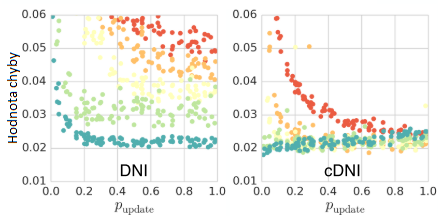
\includegraphics[width=0.6\textwidth]{images/vysledkyExperimentuBpLambda}}
%popis obrazku
\caption[Podmienenie aktivácie spätného šírenia chyby pravdepodobnosťou $p\textsubscript{update}$]{Grafy znázorňujú vývoj chyby konvolučnej neurónovej siete trénovanej na klasifikáciu dátovej sady MNIST \cite{yann1998mnist}. Neurónová sieť upravuje váhy skrytých vrstiev využitím syntetického gradientu. Po dokončení fázy dopredného šírenia sa vykoná fáza spätného šírenia chyby s pravdepodobnosťou $p_{update}$. Graf vľavo znázorňuje, aký vplyv má pravdepodobnosť aktivácie fázy spätného šírenia $p_{update}$ na chybu neurónovej siete využívajúcu syntetický gradient (DNI). Graf vpravo zobrazuje, aký vplyv má pravdepodobnosť aktivácie fázy spätného šírenia chyby $p_{update}$ na neurónovú sieť využívajúcu syntetický gradient generovaný modulom syntetického gradientu s dodatočná informácia o supervízii $c$ (cDNI) \cite{Jaderberg2016}.}
%id obrazku, pomocou ktoreho sa budeme na obrazok odvolavat
\label{vysledkyExperimentuBpLambda}
\end{figure}

\section{Rozšírenie modulu syntetického gradientu}

Na začiatku kapitoly sme opísali experiment z \cite{Jaderberg2016}, pri ktorom bola konvolučná neurónová sieť aplikovaná na klasifikáciu dátovej sady MNIST \cite{yann1998mnist}. Táto neurónová sieť vykonávala na každej skrytej vrstve lineárnu klasifikáciu realizovanú dávkovou normalizáciou \cite{Ioffe2015} a transformáciu dát pomocou ReLU (z angl. Rectified Linear Unit) \cite{Xu2015}. 

V ďalšom experimente \cite{Jaderberg2016} bola použitá podobná konvolučná neurónová sieť ktorá obsahuje tri skryté vrstvy a jednu klasifikačnú, výstupnú vrstvu. Ku každej skrytej vrstve je pripojený samostatný modul syntetického gradientu. Experiment pozoroval vplyv syntetického gradientu a hĺbky neurónovej siete na klasifikáciu rukou-písaných čísel dátovej sady MNIST a rozpoznávanie objektov dátovej sady CIFAR-10 \cite{Krizhevsky09learningmultiple}. V každom pozorovaní je hĺbka neurónovej siete menená medzi 3 až 6 skrytými vrstvami. 

Výsledok experimentu je možné vidieť v tabuľke \ref{compareDNIandCDNI}. Využitie DNI v praxi skutočne funguje \cite{Jaderberg2016}. DNI za cenu drobného poklesu presnosti predikcie, umožňuje úplne odstrániť \textit{uzamknutie úpravy váh} a \textit{uzamknutie v smere spätného šírenia chyby}. 

Experiment tiež pozoroval vplyv dodatočnej informácie o supervízii $c$ poskytnutej modulom syntetického gradientu, na presnosť predikcie neurónovej siete. Z tabuľky \ref{compareDNIandCDNI} je možné vidieť, že poskytnutím dodatočnej informácie $c$ je možné trénovať neurónovú sieť s ešte menšou degradáciou presnosti ako v prípade využitia štandardného syntetického gradientu \cite{Jaderberg2016}. Toto tvrdenie vyplýva z porovnania presnosti predikcie na dátovej sade CIFAR-10. Zatiaľ čo neurónová sieť pozostávajúca z piatich skrytých vrstiev, využívajúca štandardný syntetický gradient má chybu 46.9\%, tak tá istá neurónová sieť, využívajúca syntetický gradient generovaný s využitím dodatočnej informácie $c$ má chybu predikcie 43.5\%. 

Zdroj \cite{Jaderberg2016} nakoniec uviedol, že vykonal experiment pri ktorom trénoval neurónovú sieť ktorá mala viac ako 21 skrytých vrstiev. Táto neurónová sieť využívala výhradne syntetický gradient generovaný modulom syntetického gradientu s dostupnou dodatočnou informáciou $c$ a hodnota chyby bola 2\%.

\begin{table}
% v tabulke sa popis zvykne davat nad tabulku
\caption[Porovnanie chyby neurónovej siete trénovanej rôznymi typmi gradientu]{Tabuľka zobrazuje chybu predikcie konvulenčnej neurónovej siete trénovanej na rozpoznávanie obrazu z dátových sád MNIST a CIFAR-10. Prvý stĺpec udáva informáciu o hĺbke neurónovej siete, kde daná hodnota predstavuje počet skrytých vrstiev. Pre každú dátovú sadu bola použitá tá istá neurónová sieť. Tabuľka obsahuje hodnoty chyby neurónovej siete využívajúcej gradient šírený spätnou propagáciou chyby (Bprop), syntetický gradient (DNI) alebo syntetický gradient obohátený o dodatočnú informáciu $c$ (cDNI) \cite{Jaderberg2016}.}
%id tabulky
\label{compareDNIandCDNI}
% tu zacina samotna tabulka
\begin{center}
\begin{tabular}{cc|ccc|ccc}
\toprule
      &       & \multicolumn{3}{c|}{MNIST (\% Chyba)} & \multicolumn{3}{c}{CIFAR-10 (\% Chyba)} \\
\midrule
\multicolumn{2}{c|}{Počet vrstiev} & Bprop & DNI  & cDNI  & Bprop & DNI & cDNI \\ \hline
\hline
\multicolumn{2}{c|}{3} & 2,0 & 1,9 & 2,2 & 43,5 & 42,5 & 48,5 \\
\multicolumn{2}{c|}{4} & 1,8 & 2,2 & 1,9 & 43,0 & 45,0 & 45,1 \\
\multicolumn{2}{c|}{5} & 1,8 & 3,4 & 1,7 & 41,7 & 46,9 & 43,5 \\
\multicolumn{2}{c|}{6} & 1,8 & 4,3 & 1,6 & 42,0 & 49,7 & 46,8 \\
\hline
%(many lines omitted)
\bottomrule
\end{tabular}%
\end{center}
\end{table}

Na tento experiment sme sa zamerali predovšetkým preto, aby sme zistili aký vplyv má syntetický gradient na neurónovú sieť, ktorá vykonáva lineárnu klasifikáciu realizovanú dávkovou normalizáciou a ReLU. Skutočnosť, že implementácia syntetického gradientu na takýto typ neurónovej siete nemá signifikantne negativný vplyv na presnosť neurónovej siete je pre nás pozitívna. Pozitívna vzhľadom k tomu, že ďalšia časť práce sa bude venovanáť reziduálnym sieťam ktoré využívajú dávkovú normalizáciu a ReLU. V tomto ohľade je pre nás nevyhnutné disponovať informáciou o tom, aký efekt syntetického gradientu na takúto sieť máme očakávať.

\chapter{Experimenty modifikácie reziduálneho bloku}

\section{Vplyv architektúry reziduálneho bloku na reziduálnu sieť}

\begin{table}[h]
% v tabulke sa popis zvykne davat nad tabulku
\caption[Porovnanie architektúr reziduálneho bloku]{Pozorovanie vplyvu architektúry reziduálneho bloku na chybu predikcie reziduálnej siete. Pozorovanie bolo vykonané na dvoch reziduálnych sieťach. Reziduálna sieť so 110 skrytými konvolučnými vrstvami (ResNet-110) a reziduálna sieť so 164 skrytými konvolučnými vrstvami (ResNet-164). Obidve neurónové siete boli trénované na rozpoznávanie obrazu z dátovej sady CIFAR-10 \cite{He2016}. Vizualizáciu pozorovaných architektúr reziduálnych blokov je možné vidieť na Obrázku \ref{fig:architectures_of_residual_blocks}}
%id tabulky
\label{compareArchitectures}
% tu zacina samotna tabulka
\begin{center}
\begin{tabular}{l|c|c|c}
\toprule
\multicolumn{2}{c}{} & \multicolumn{2}{c}{chyba (\%)} \\
\midrule
Architektúra & Obrázok & ResNet-110  & ResNet-164\\ \hline
\hline
pôvodný reziduálny blok          & Obr. \ref{fig:architectures_of_residual_blocks} a) & 6,61 & 5,93 \\
dávková normalizácia po sčítaním & Obr. \ref{fig:architectures_of_residual_blocks} b) & 8,17 & 6,50 \\
ReLu pred sčítaním               & Obr. \ref{fig:architectures_of_residual_blocks} c) & 7,84 & 6,14 \\
ReLu predaktivácia               & Obr. \ref{fig:architectures_of_residual_blocks} d) & 6,71 & 5,91 \\
\textbf{úplná predaktivácia}     & Obr. \ref{fig:architectures_of_residual_blocks} e) & \textbf{6,37} & \textbf{5,46} \\
\hline
%(many lines omitted)
\bottomrule
\end{tabular}%
\end{center}
\end{table}
\newpage

\section{Vplyv architektúry identitného prepojenia na reziduálnu sieť}

\begin{table}[h]
% v tabulke sa popis zvykne davat nad tabulku
\caption[Porovnanie rôznych architektúr identitného prepojenia]{Porovnanie vplyvu transformácie identického zobrazenia prechodom identitným prepojením na presnosť reziduálnej siete. Pozorovaná reziduálna sieť bola trénovaná na rozpoznávanie obrazu z dátovej sady CIFAR-10. Pozostávala zo 110 skrytých konvolučných vrstiev (ResNet-110) obsahujúcich $3\times 3$ konvolučné filtre. Niektoré merania boli vykonané viackrát, s rôznymi počiatočnými hodnotami preferencií $b_g$ (z angl. bias). Slovo \textit{zlyhanie} je použité, ak hodnota chyby presiahla 20\% \cite{He2016}. Vizualizácia pozorovaných architektúr identitného prepojenia je možné vidieť na Obrázku \ref{fig:achitectures_of_identity_shortcut}.}
%id tabulky
\label{compareIdentityTransformations}
% tu zacina samotna tabulka
\begin{comment}
\begin{center}
\begin{tabular}{l|c|c|c|c|l}
\toprule
Architektúra    & Obrázok  & na prepojení   &  na $\mathcal{F}$    & chyba (\%) & poznámka \\ 
\hline
\hline
pôvodný & Fig \ref{fig:achitectures_of_identity_shortcut}(a) & 1 & 1 & \textbf{6,61} & \\
\hline
\multirow{3}{*}{constant scaling}   & \multirow{3}{*}{Fig \ref{fig:achitectures_of_identity_shortcut}(b)} & 0 & 1 & zlyhanie & \\
& & 0,5 & 1 & zlyhanie & \\
& & 0,5 & 0,5 & 12,35 &  \\
\hline
\multirow{3}{*}{exclusive gating}   & \multirow{3}{*}{Fig \ref{fig:achitectures_of_identity_shortcut}(c)} & $1-g(x)$ & $g(x)$ & zlyhanie & $b_g = 0$ to $5$\\
& & $1-g(x)$ & $g(x)$ & 8,70 & $b_g = -6$\\
& & $1-g(x)$ & $g(x)$ & 9,81 & $b_g = -7$\\
\hline
\multirow{2}{*}{shortcut-only gating}   & \multirow{2}{*}{Fig \ref{fig:achitectures_of_identity_shortcut}(d)} & $1-g(x)$ & 1 & 12,86 & $b_g = 0$\\
& & $1-g(x)$ & 1 & 6,91 & $b_g = -6$\\
\hline
$1\times1$ conv shortcut& Fig \ref{fig:achitectures_of_identity_shortcut}(e) & $1\times1$ conv & 1 & 12,22 \\
\hline
dropout shortcut & Fig \ref{fig:achitectures_of_identity_shortcut}(f) & dropout 0,5 & 1 & zlyhanie \\
\hline
%(many lines omitted)
\bottomrule
\end{tabular}%
\end{center}
\end{comment}

\begin{center}
\begin{tabular}{l|c|c|l}
\toprule
Architektúra    & Obrázok  & chyba (\%) & poznámka \\ 
\hline
\hline
pôvodné identitné prepojenie & Obr. \ref{fig:achitectures_of_identity_shortcut} a) & \textbf{6,61} & \\
\hline
konštantné škálovanie   & Obr. \ref{fig:achitectures_of_identity_shortcut} b) & 12,35 &  \\
\hline
\multirow{3}{*}{exkluzívne hradlovanie}  & \multirow{3}{*}{Obr. \ref{fig:achitectures_of_identity_shortcut} c)} & zlyhanie & $b_g = 0$ to $5$\\
& & 8,70 & $b_g = -6$\\
& & 9,81 & $b_g = -7$\\
\hline
\multirow{2}{*}{hradlovanie v rámci prepojenia}   & \multirow{2}{*}{Obr. \ref{fig:achitectures_of_identity_shortcut} d)} & 12,86 & $b_g = 0$\\
& & 6,91 & $b_g = -6$\\
\hline
$1\times1$ konvulenčné prepojenie & Obr. \ref{fig:achitectures_of_identity_shortcut} e) & 12,22 \\
\hline
stochastické vynechávanie prepojenia (dropout)& Obr. \ref{fig:achitectures_of_identity_shortcut} f) & zlyhanie & \\
\hline
%(many lines omitted)
\bottomrule
\end{tabular}%
\end{center}

\end{table}

\chapter{Plán práce na riešení projektu}
\begin{enumerate}
    \item Implementácia metódy DeepCyTOF (December)
    \item Implementácia syntetického gradientu v reziduálnej sieti MMD-ResNet (Január-Február)
    \item Experimentovanie a pozorovanie vplyvu syntetického gradientu na presnosť predikcií metódy DeepCyTOF (Marec)
    \item Vyhodnocovanie experimentov (Apríl)
\end{enumerate}